\documentclass{amsart}
\usepackage[pdftex]{graphicx}

\title{Modeling Intervention Strategies for United States TB Control}
\begin{document}
\maketitle

\section{Introduction}
Epidemiological models allow public health professionals to predict and analyze
disease dynamics and intervention effectiveness. The most common examples of
such models are compartmental differential equation models, in which the
population is split between several possible health states, with flow between
each state given according to deterministic differential equations. In 2012, 
Hill, Becerra, and Castro implemented a compartmental
differential equaiton model of tuberculosis (TB) in the United States (US).
Their model utilized five health states and two subpopulations, US-born (USB)
and foreign-born (FB) for a total of 10 compartments. They used this model to
evaluate several possible intervention strategies, and ultimately conclude that
though increasing LTBI treatment was a good intervention strategy, the US was
unlikely to meet their stated goal of elimination of TB in the US by 2100. In
this work, the Hill model was extended in several key ways. First, additional
tracking capabilities were added to the Hill model, such that it can now report
further granularity in the disease dynamics. Further, economic components were
added to the model in order to project the US health care system (HCS) costs due
to TB given our current policy as well as for various interventions. Finally, a
population level, agent based implementation of the Hill Model was created, in
order to validate the Hill Model against the natural stochasticity present in
real world disease spread. 

\section{Background}

\subsection{The Hill Model}
A flowchart representation of the Hill Model is shown in Figure 1.  Each compartment
represents a different possible health state with respect to TB for every 
US-born or foreign-born individual, and arrows between different compartments
represent possible transitions between states.  Individuals also leave the model 
from all compartments due to natural death, which is left out of the figure for clarity.  \\

\begin{figure}
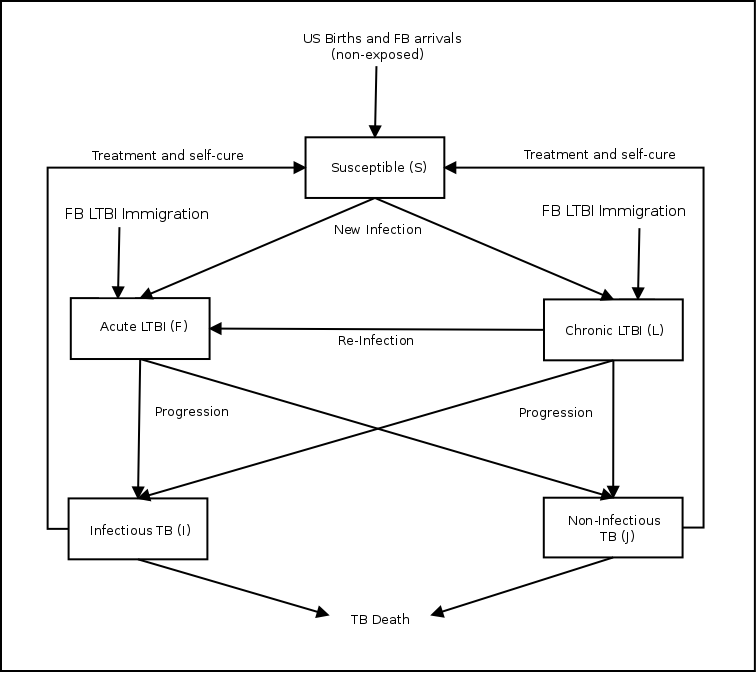
\includegraphics[scale=0.25]{figures/HillModelFlowChart.png}
\end{figure}

The majority of USB and FB individuals fall into the Susceptible (S) category, which includes everyone
who is uninfected and has not been exposed to TB.  After exposure to an individual
with TB, a person in the Susceptible compartment can develop Latent TB Infection (LTBI) and changes
health states to either the Acute LTBI (F) or Chronic LTBI (L) compartment.  Latently
infected individuals are not infectious, but have some risk of developing active TB infection
over time.  However, the rates of disease progression are not equal, and individuals in the
Acute LTBI compartment have a higher risk of developing active TB than those in
the Chronic LTBI compartment.  Individuals in the Chronic LTBI compartment
may also be exogenously re-infected and transition to the Acute LTBI compartment.  \\

Latently infected individuals may progress to one of two active TB states: Infectious TB (I) or 
Non-Infectious TB (J).  Individuals in both compartments have an increased risk of death from
active TB infection, but only individuals in the Infectious TB compartment are contagious.  
In addition, individuals in all of the infected compartments (F, L, I, J) may be treated or self-cure
themselves of their respective TB health condition.  However, in the model, treatment or self-cure from TB
does not grant immunity, and all healthy individuals are grouped in the Susceptible compartment
and may be re-infected at a later time.  \\

\section{Methods}

\subsection{Basic Implementation}
Both the basic Hill Model and this extended Hill Model were implemented in
\texttt{R} as a system of differential equations, which were solved via the
$\texttt{lsoda}$ routine. The systems of differential equations used in the Basic
Hill Model and the extended Hill Model are shown below in Figure 2 and Figure 3
respectively.   

\begin{figure}
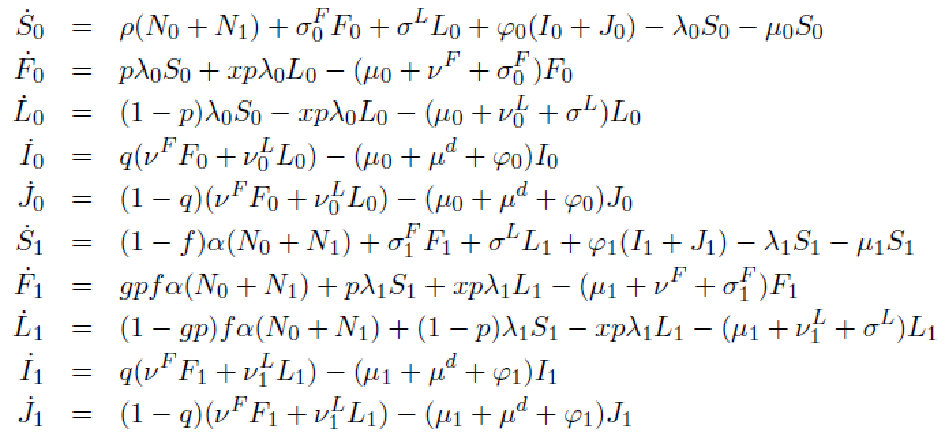
\includegraphics[scale=0.75]{figures/BasicHillEquations.pdf}
\end{figure}

The vector variables $S_{0}, F_{0}, L_{0}, I_{0}, J_{0}$ contain the number of US-born individuals in the S, F, L, I, J compartments respectively, and $S_{1}, F_{1}, L_{1}, I_{1}, J_{1}$ contain foreign-born individuals.  $N_{0}$ and $N_{1}$ are the total populations of US-born and foreign-born individuals.
The constants $\rho$ and $\alpha$ are birth rates, while $\mu_{i}$, and $\mu_{d}$ are death rates.  
A complete list and descriptions of all constants used in the model can be found in the appendix.

\subsection{Additional Tracking Capabilities}
In order to refine the tracking capabilities of the
Hill Model, the original differential equations used to describe TB spread were
separated into their component parts and each section was tracked separately.
These components were made into compartments, tracked by differential equations
EQUATION NUMBER SOMETHING TO SOMETHING, SORTED BY COMPARTMENT. In addition,
estimations of the basic reproductive number of FB or USB active, infectious TB
cases were made from a theoretical and an experimental perspective. Experimental
data were calculated by reducing the initial population of FB or USB active,
infectious TB cases by 1 and predicting the final number of cases seen in each
case, in $\texttt{R}$. 

\subsection{Economic Modeling}
Further, estimates for the cost of active TB treatment and for the cost of
latent TB infection (LTBI) treatment were obtained from Dylan et. al. and So and
So adherence effectivenss. CITE ME!
Both these costs and any health state outcomes were discounted at a rate of 3\%
per year. From these estimated cost per treatment, total costs were obtained in
the following way. It was assumed that every patient in the US with active TB is
treated, not necessarily successfully, but further that every treatment costs
exactly the average cost per treatment. Thus, active TB costs could be tracked
simply by tracking the number of new active TB cases, and scaling by a
discounted cost per treatment rate. Given the structure of the model, further
granularity was obtained from the cost data by tracking separately the cost due
to new cases that stemmed from activation of a chronic LTBI case, or activation
of an acute LTBI case. These values give estimates for the US HCS TB cost due to
exogenous infection of TB vs the US HCS TB cost due to activation of LTBI. Each
of these components of the cost was a new differential equation tracked by the
model, also solved by $\texttt{lsoda}$. For LTBI treatment cost, treatment was
charged upon leaving the LTBI compartment due to the cumulative self-cure and
treatment rate given in the Hill Model. The fraction of these indviduals who
leave this compartment due to self cure was assumed to be zero. Given the
uncertainty in measurments of LTBI treatment cost, extensive sensitivity
analysis was performed on this parameter relative to final cost outcomes, which
showed that it had an XXXXXXXXX effect. In addition to US HCS cost, the system
was implemented so as to also track projected intervention implementation cost,
given user-inputted parameters relating to various possible intervention cost
strategies. The extended Hill Model was used to track the effect of many
interventions tested by the Hill Model as well as an additional intervention
strategy of curing cases of immigrating LTBI prior to entry. This intervention
strategy proved very promising and elimination year, final cost, and cost per
case averted were tracked for various levels of entering LTBI cure rate. The
interventions were implemented so as to take effect during the year 2013 and run
to 2100. The numerical DE solver $\texttt{lsoda}$ used was run with a time step
of $0.8$. Sensitivity analysis was performed on this parameter and reducing the
time step was shown to have minimal effect on final size or cost values. 

\subsection{Agent Based}
The population level agent based model was implemented in several ways. Early
implementations were built in \texttt{Netlogo} and \texttt{Java}, but final
implementations were constructed in $\texttt{C++}$. An implementation was made
that tracked the hill model exactly, up to still including the Acute Latent
compartment in the model. Probabilites of agent progression between various
health states were computed given rates in the hill model and a variety of
approximations. The final size standard deviation and distribution data was
collected via 2160 (MINUS SOME) runs with each agent in the model truly
representing one individual and a time step of $0.01$. These data were analyzed
in $R$. 

\section{Results}

\subsection{Basic Population Breakdown}
The additional tracking capabilities offered several key insights into US TB
dynamics. Figure INSERT FIGURE HERE shows the yearly incidence of US TB, broken
down into infeciton source. It can be seen that the majority of the US TB load
is driven by activations of FB LTBI, followed by USB LTBI activations. This data
further agrees with the conclusions drawn by Hill, Becerra, and Castro about the
necessity of LTBI treatment in any valuable intervention strategy. Further,
figure INSERT FIGURE HERE shows a similarly sourced plot, but analyzing the
final US HCS costs due to TB. One can see that in this plot, roughly half of the
US TB HCS costs are due to activations of LTBI. Note that both of these plots
underestimate the impact LTBI activations play in the spread of TB, as every
LTBI activation to infectious TB contributes not only to incidence and costs
directly, but also indirectly by causing additional future cases, which is not
captured in these graphs. 
\subsubsection{Basic Reproduction Number}
The basic reproduction number of FB or USB cases of infectious TB was also
estimated by this system. From a theoretical perspective, we can think of the
total number of secondary infections over 100 years due to a FB or USB
infectious TB case as describing a geometric series in a large population.
Presuming there are no overlaps in infectious contacts, if a single case of
infectious TB in either population infects $p_f, p_u$ new cases in one year,
respectively, then we can say that over the course of 100 years, the total
number of cases infected will follow a geometric series. This analysis predicts
that over 100 years, one USB individual will infect $1.03$ other individuals,
whereas one FB individual will infect $.64$ other individuals. Experimentally,
these data were also analyzed, with results of $1.04$ and $.8$, respectively. 

\subsection{Intervention Analysis}
The primary interventions analyzed by the extended Hill were those that analyzed
curing various percentages of entering LTBI cases. Four indicative percentages
chosen were $20\%$, $35\%$, $50\%$, and $65\%$. Note that the hill model does
not distinguish documented immigration from undocumented immigration, and as
such estimates of entering LTBI cure rates higher than $65\%$ become much more
difficult to acheive. 

\subsection{Agent Based Evaluation}
\subsection{Sensitivity Analysis}
\end{document}
